\section{Visual encoder finetuning}
\label{sec:visual-encoder-finetuning}


\begin{figure*}[t]
  \centering
    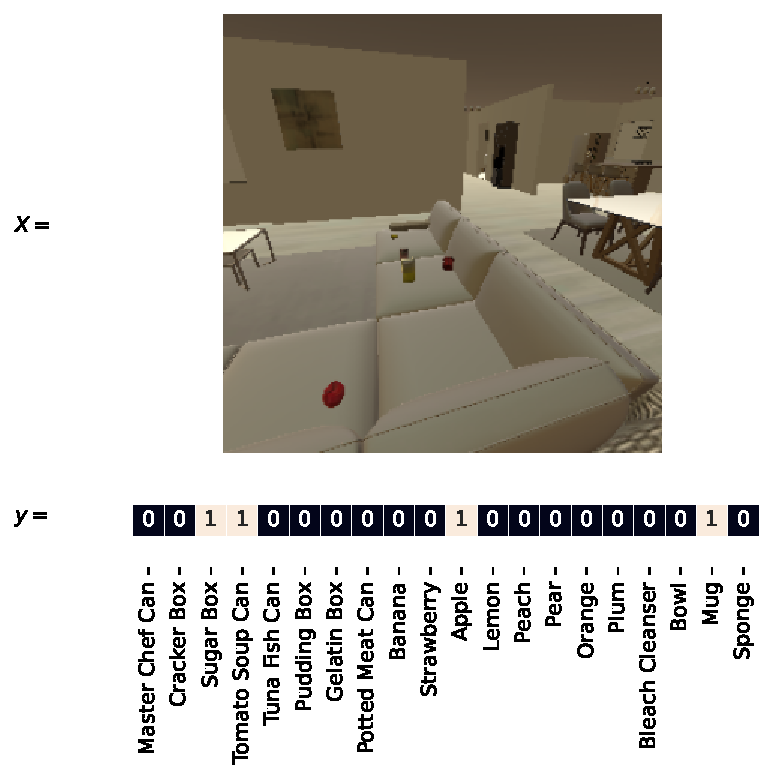
\includegraphics[width=0.5\textwidth]{figures/results/finetuning_smaple.pdf}
    \caption{Sample of the finetuning data}
  \label{fig:finetuning_data}
\end{figure*}

We finetuned the visual encoder on a generated supervised task before freezing it to be used in our experiments. 
Each sample, \Cref{fig:finetuning_data}, in the data is generated by placing the agent in front of a random object then the RGB sensor data is used as input $X$. The output $y$ is a binary vector of size 20, the number of available object types, where each element represents whether the corresponding object type is in the image or not. The object type is considered in the image if there is an instance of this object in the image with more than 10 pixels. 
21k samples are generated from the training scenes and object arrangements. The 21k samples are then split to training and validation data with ratios 90\% to 10\%.

The VC-1 model is finetuned using the Dice loss \cite{Sudre_2017_diceloss} by adding a classification head to the output of `[CLS]' token using the generated data. The classification head is first finetuned for 5 epochs with $LR=0.001$ while the remaining of the model is frozen. Then the model is unfrozen and finetuned for 15 epochs with $LR=0.00002$.
\gc{Maybe add a citation for this strategy here. \\ Ahmad: What strategy? }
